\documentclass[a4paper, 12pt]{article}
\usepackage[portuguese]{babel}
\usepackage[utf8]{inputenc}
\usepackage{amsmath}
\usepackage{enumerate}
\usepackage[pdftex]{hyperref}
\usepackage{graphicx}
\usepackage{placeins}
\usepackage{listings}
\lstset{language=Java}
\renewcommand{\lstlistingname}{Código}
\hypersetup{
  colorlinks,
  citecolor=blue,
  filecolor=blue,
  linkcolor=red,
}
\title{UFSC / CTC / INE \\
{\bf Disciplina: Introdução à Internacionalização de Software} \\
{\bf Relatório do Trabalho Prático}}

\author{ {\bf Curso de Sistemas de Informação: INE5653-07238}  \\
  Vitor Arins  \\
  Matrícula: 12205530
}

\date{\today}
\begin{document}
\maketitle

\begin{abstract}
Este documento tem como objetivo tratar de forma acadêmica os
procedimentos na internacionalização de um software chamado ``Game Of
Pig''. O software se trata de um jogo de dados virtual. Este trabalho
irá relatar o passo a passo do processo de tornar o software acessível
em pelo menos duas línguas diferentes. Será apresentado a fase
anterior a internacionalização, os procedimentos e a fase seguinte ao
processo.
\end{abstract}

\section{Antes} \label{antes}

\FloatBarrier
\paragraph{} Antes do processo de internacionalização, a interface visual
apresentava apenas a linguagem português, como é possível observar na
Figura 1.

\begin{figure}[h!]
\centering
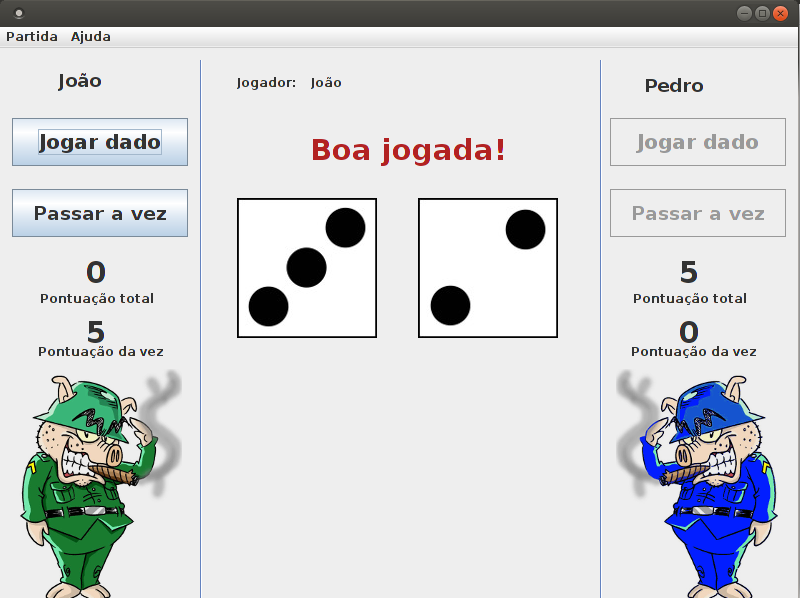
\includegraphics[width=\textwidth]{pig-portugues.png}
\caption{Interface anterior}
\end{figure}

\FloatBarrier
\paragraph{} Além da interface estar localizada apenas para português
do Brasil, o texto utilizado estava programado direto como
\emph{String} nos componentes, tornando a iternacionalização do
software ainda mais difícil. Assim ilustrado na passagem de código a
seguir:

\begin{lstlisting}[frame=single, caption={Código anterior},
  captionpos=b]

protected JMenu mnPartida = 
          new JMenu("Partida");
protected JMenuItem mntmConectar = 
          new JMenuItem("Conectar");
protected JMenuItem mntmIniciarPartida = 
          new JMenuItem("Iniciar Partida");
protected JMenuItem mntmDesconectar = 
          new JMenuItem("Desconectar");
protected JButton btnJogarDado1 = 
          new JButton("Jogar dado");

\end{lstlisting}

\section{Procedimentos} \label{procedimentos}
Para resolver o problema, foram utilizadas algumas ferramentas.

\FloatBarrier
\subsection{Extração} \label{extraction}

\paragraph{} Primeiro foi utilizada a função \emph{Externalize
  Strings...} presente no \emph{Eclipse} para identificar todas as
\emph{Strings} do código, associar uma {\bf chave} a cada valor de
\emph{String} e criar um arquivo do tipo {\bf \emph{.properties}} para
guardar essas chaves e valores.

\begin{figure}[h!]
\centering
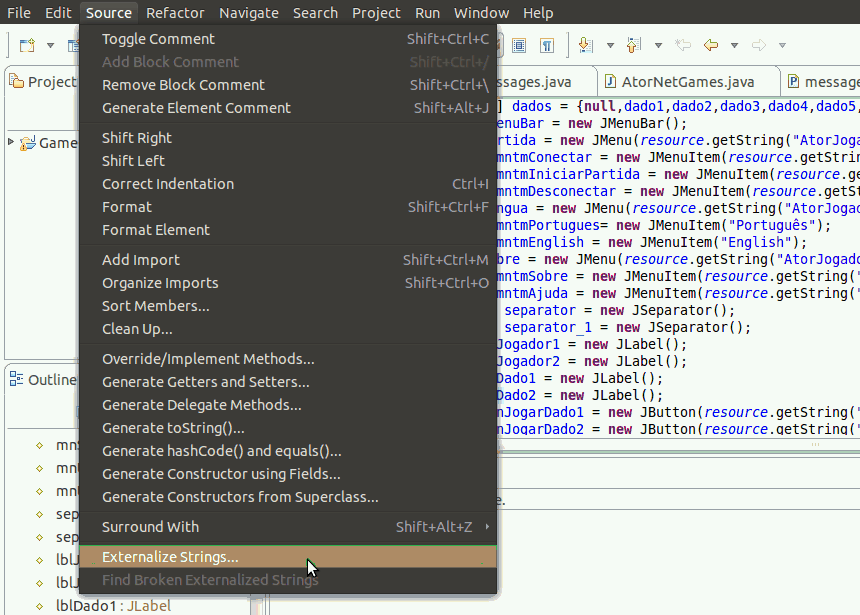
\includegraphics[width=\textwidth]{Screenshot-externalize.png}
\caption{\emph{Externalize Strings...}}
\end{figure}

\FloatBarrier
\subsection{Edição} \label{edition}

\paragraph{} Em seguida foi utilizado um editor de arquivos do tipo
{\bf \emph{.properties}} que vem como plugin do \emph{Eclipse} chamado
\emph{ResourceBundle Editor}.

\begin{figure}[h!]
\centering
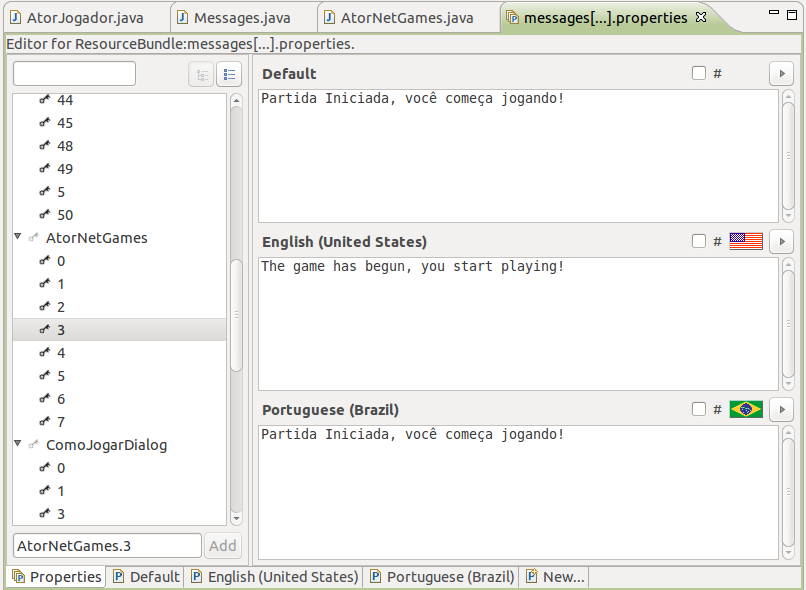
\includegraphics[width=\textwidth]{Screenshot-rbeditor.png}
\caption{\emph{ResourceBundle Editor}}
\end{figure}

\FloatBarrier
\subsection{Utilização} \label{use}

\paragraph{} Para utilizar o novo arquivo gerado, é necessário criar
um objeto Java da classe {\bf \emph{ResourceBundle}}, passando o nome
do arquivo de mensagens e a localização atual do usuário:

\begin{lstlisting}[frame=single, caption={Criando ResourceBundle},
  captionpos=b]
private final String BUNDLE_NAME = "pig.messages";
protected static ResourceBundle resource =
                 ResourceBundle.getBundle(BUNDLE_NAME,
                                  Locale.getDefault());
\end{lstlisting}

\paragraph{} Em seguida o objeto é utilizado para recuperar {\bf
  Strings} a partir da chave referente:

\begin{lstlisting}[frame=single, caption={Uso ResourceBundle},
  captionpos=b]
protected JMenu mnPartida = new
          JMenu(resource.getString("AtorJogador.11"));
\end{lstlisting}

\section{Resultados} \label{results}

\FloatBarrier
\paragraph{} Ao final dos procedimentos para internacionalização do
software, é possível executar o jogo e a interface irá se adaptar ao
local definido na máquina em que está sendo executado.

\begin{figure}[h!]
\centering
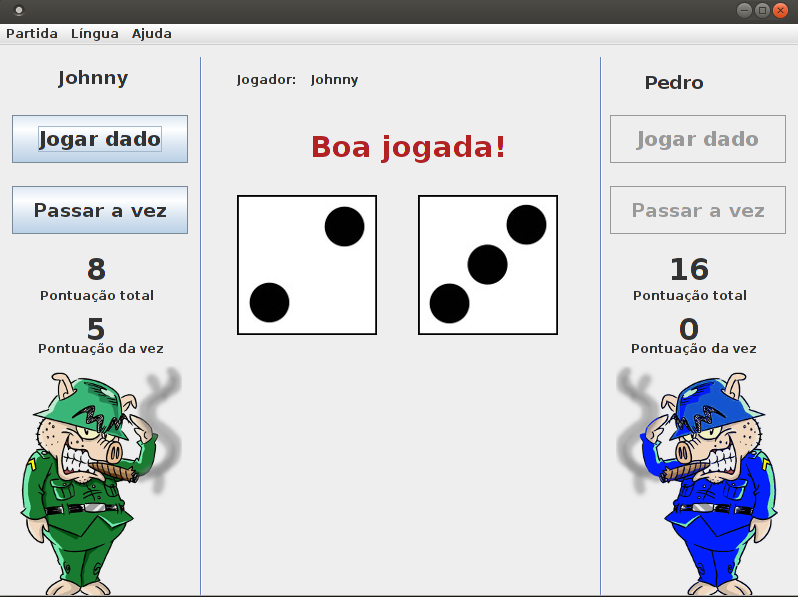
\includegraphics[width=\textwidth]{Screenshot-portugues.png}
\caption{\emph{Jogo em português}}
\end{figure}

\begin{figure}[h!]
\centering
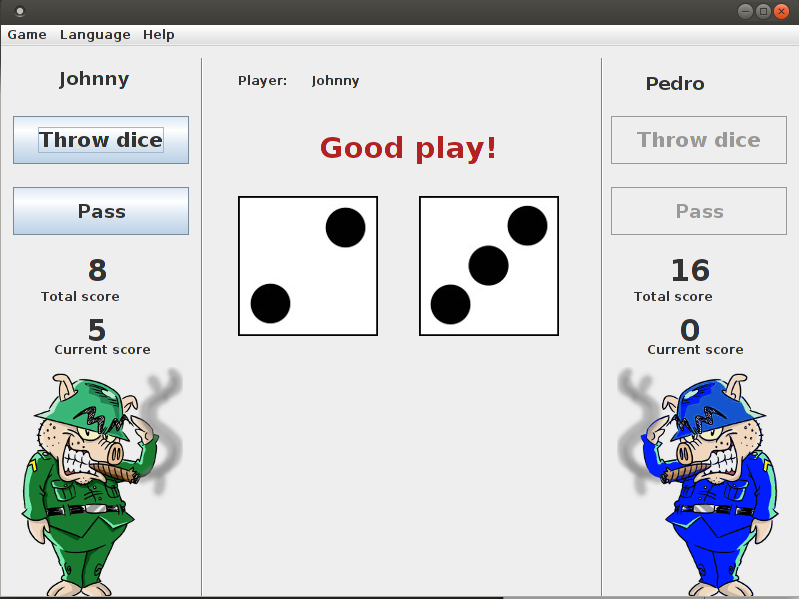
\includegraphics[width=\textwidth]{Screenshot-ingles.png}
\caption{\emph{Jogo em inglês}}
\end{figure}

\FloatBarrier
Também foi adicionado um botão para alterar a linguagem
caso necessário durante a execução do jogo.
\begin{figure}
\centering
\begin{minipage}{.5\textwidth}
\centering
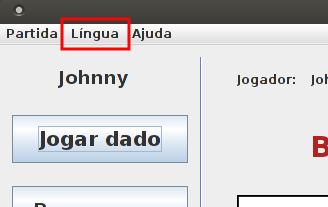
\includegraphics[scale=0.4]{Screenshot-lingua.png}
\caption{\emph{Escolha da linguagem}}
\end{minipage}%
\begin{minipage}{.5\textwidth}
\centering
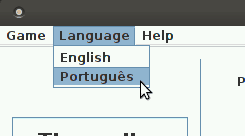
\includegraphics[scale=0.6]{Screenshot-menulingua.png}
\caption{\emph{Menu da linguagem}}
\end{minipage}
\end{figure}

\FloatBarrier
\paragraph{} Para realizar esta alteração, foi necessário criar um
método de mudança da localização que define novamente o texto de cada
componente após o clique.

\begin{lstlisting}[frame=single, caption={Clique no Menu de Linguagem},
  captionpos=b]
mntmEnglish.addActionListener(new ActionListener() {
  public void actionPerformed(ActionEvent e) {
    Locale.setDefault(Locale.US);
    changeLocale();
  }
});
mntmPortugues.addActionListener(new ActionListener() {
  public void actionPerformed(ActionEvent e) {
    Locale.setDefault(new Locale("pt_BR"));
    changeLocale();
  }
});
\end{lstlisting}

\begin{lstlisting}[frame=single, caption={Método de definição das
    novas \emph{Strings}}, captionpos=b]
protected void changeLocale() {
  resource = 
    ResourceBundle.getBundle(BUNDLE_NAME,
      Locale.getDefault());
  mnPartida.setText(
    resource.getString("AtorJogador.11"));
  mntmConectar.setText(
    resource.getString("AtorJogador.12"));
...
}
\end{lstlisting}

\end{document}